
\chapter[Suporte Tecnológico]{Suporte Tecnológico}

O objetivo desta seção é explicitar todo o aparato tecnológico a nível de software que foi utilizado durante o desenvolvimento deste trabalho.  Esta seção está dividida em Ferramentas para Programação e Ferramentas de Gerenciamento .

\section{Ferramentas de Programação} % (fold)

\label{sec:engenharia_de_software}
	Neste tópico, serão apresentadas ferramentas e tecnologias voltadas ao contexto da Engenharia de Software que são utilizadas durante este trabalho, como, por exemplo, ferramentas para gerência de configuração e versionamento dos artefatos gerados.

	\subsection{GIT} % (fold)
	\label{sub:git}
	
		A ferramenta GIT\footnote{https://git-scm.com/} foi desenvolvida por Linus Torvalds durante a criação do Kernel Linux, pois Linus percebeu que existia a necessidade de criar uma ferramenta \textit{open-source} que fizesse o controle de versão \cite{bento_alise_2013}. 
		\\	O motivo para escolha da ferramenta se deve ao fato de que o Git contém o suporte para desenvolvimento linear o que garante um paralelismo de diversas áreas do desenvolvimento. Outro diferencial do Git está nos \textit{snapshots} dos objetos que são armazenados, isso significa que o Git não rearmazena arquivos que não foram alterados \cite{martinho_git_2013}.
	% subsection git (end)

	\subsection{Github} % (fold)
	\label{sub:github}
		O Github\footnote{https://github.com} é um repositório \textit{online} que fornece a criação de projetos públicos gratuitos. A ferramenta também provê um sistema de gestão para acompanhamento do desenvolvimento envolvendo um sistema de \textit{logs}, gráficos de visualização e uma \textit{Wiki} integrada a cada projeto \cite{martinho_git_2013}.
	
	 O principal motivo pela escolha do Github é que deseja-se disponibilizar a solução futuramente para consulta e aprimoramento de pessoas interessadas. 		
	% subsection github (end)

	\subsection{SonarQube}
	\label{sub:sonarqube}
	O SonarQube é uma ferramenta \textit{open-source} de analise estática de código-fonte que foca em analisar sete ramos da qualidade de código como pode ser visto na figura \ref{img:sonar}. A ferramenta apresenta métricas quanto a duplicação de código, testes unitários, complexidade, \textit{bugs} em potencial, regras da linguagem, comentários e arquitetura e design \cite{sonar}. A ferramenta foi escrita em Java e seu foco está em lidar com defeitos de código, contudo existe uma diversidade de plugins enorme que extende as funcionalidades da ferramenta \cite{ferenc_source_2014}.
\graphicspath{{figuras/}}
\begin{figure}[h]
\centering
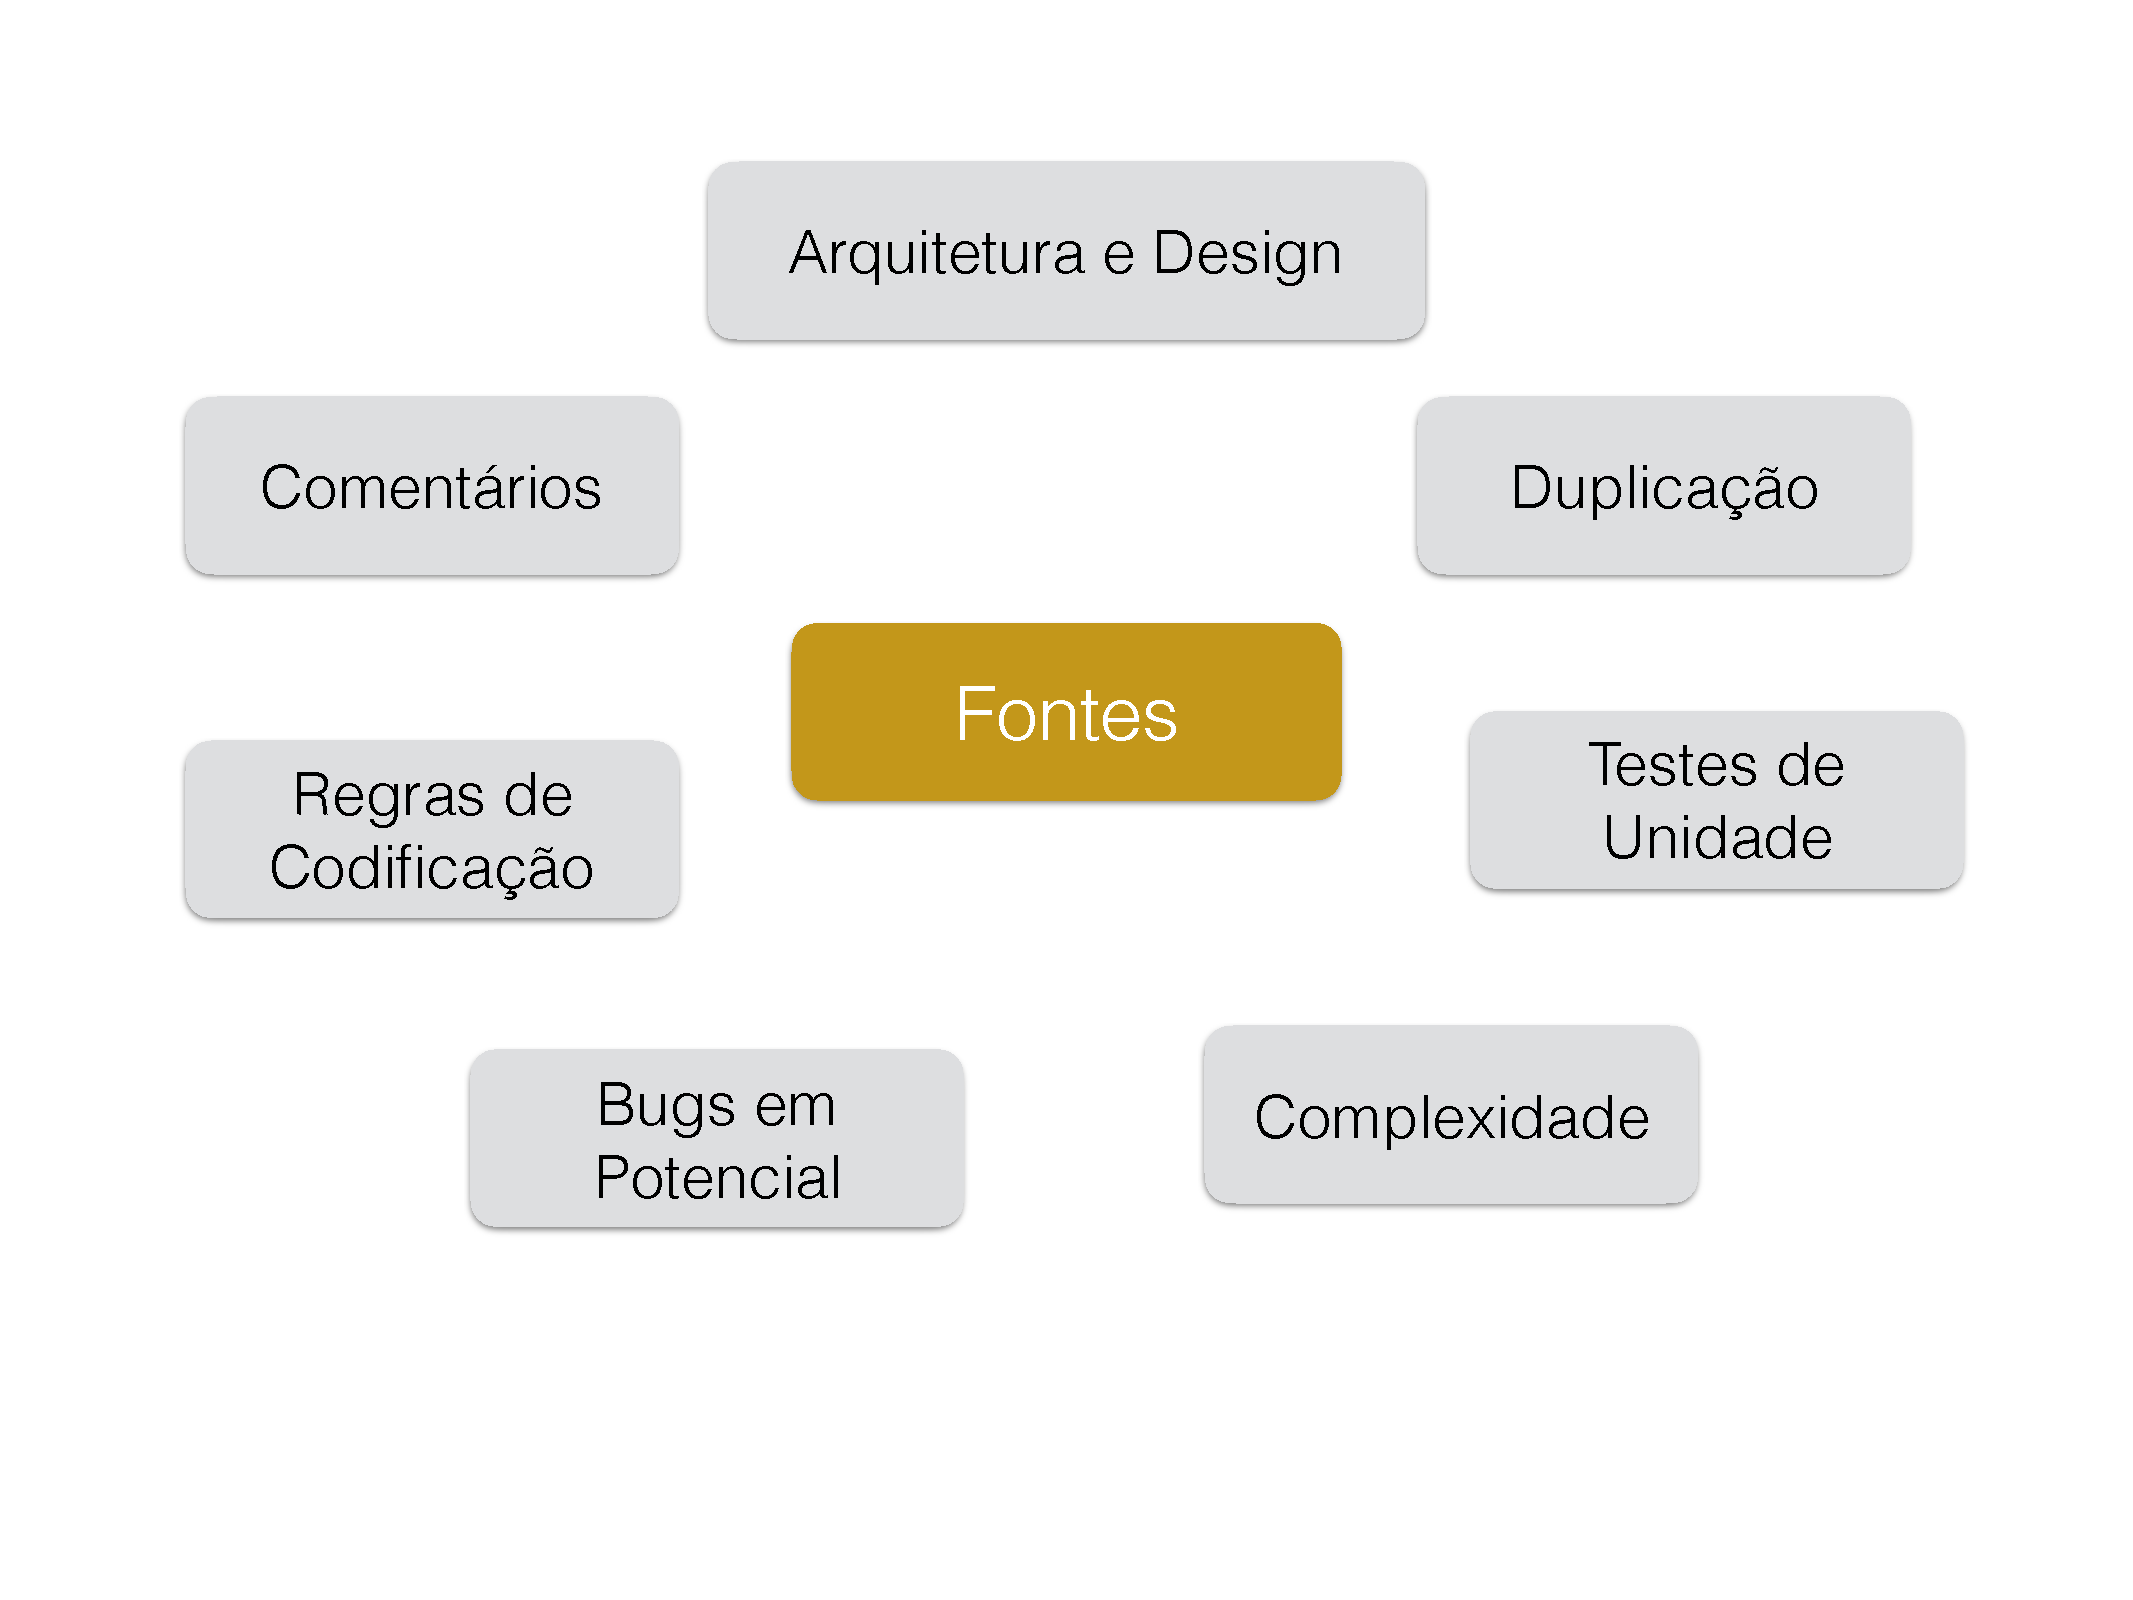
\includegraphics[scale=0.5]{Sonar}
\caption{Sete  aspectos de qualidade de código cobertos pelo SonarQube. Fonte: \cite{sonar}}
\label{img:sonar}
\end{figure}
A arquitetura do SonarQube é composta de quatro componentes como pode ser visto na figura \ref{img:arq_sonar}\cite{sonar}.
\begin{enumerate}
\item \textbf{\textit{SonarQube Server}} composto de três atividade principais:
	\begin{enumerate}
	\item Um \textbf{\textit{Web Server}} para os desenvolvedores, gerentes que procuram \textit{snapshots} da qualidade do código, e configurar uma instancia do SonarQube.
	\item Um \textbf{\textit{Search Server}} que se baseia no conceito de \textit{Elasticsearch} para devolver as buscas para a UI.
	\item Um \textbf{\textit{Compute Engine Search}} responsável pelo processamento de relatórios de análise de código e  de salvá-los no banco de dados SonarQube.
	\end{enumerate}
\item Um \textbf{SonarQube Database} que armazena a configuração da instancia do SonarQube e os \textit{snapshots} de qualidade dos projetos.
\item \textbf{Plugins} que são instalados no servidor, normalmente são plugins de linguagem, integração com outras ferramentas, autenticações entre outros.
\item Um ou mais \textbf{\textit{SonarQube Scanners}} que rodam na \textit{build} ou nos servidores de integração contínua para analisar projetos.
\end{enumerate}
\graphicspath{{figuras/}}
\begin{figure}[h]
\centering
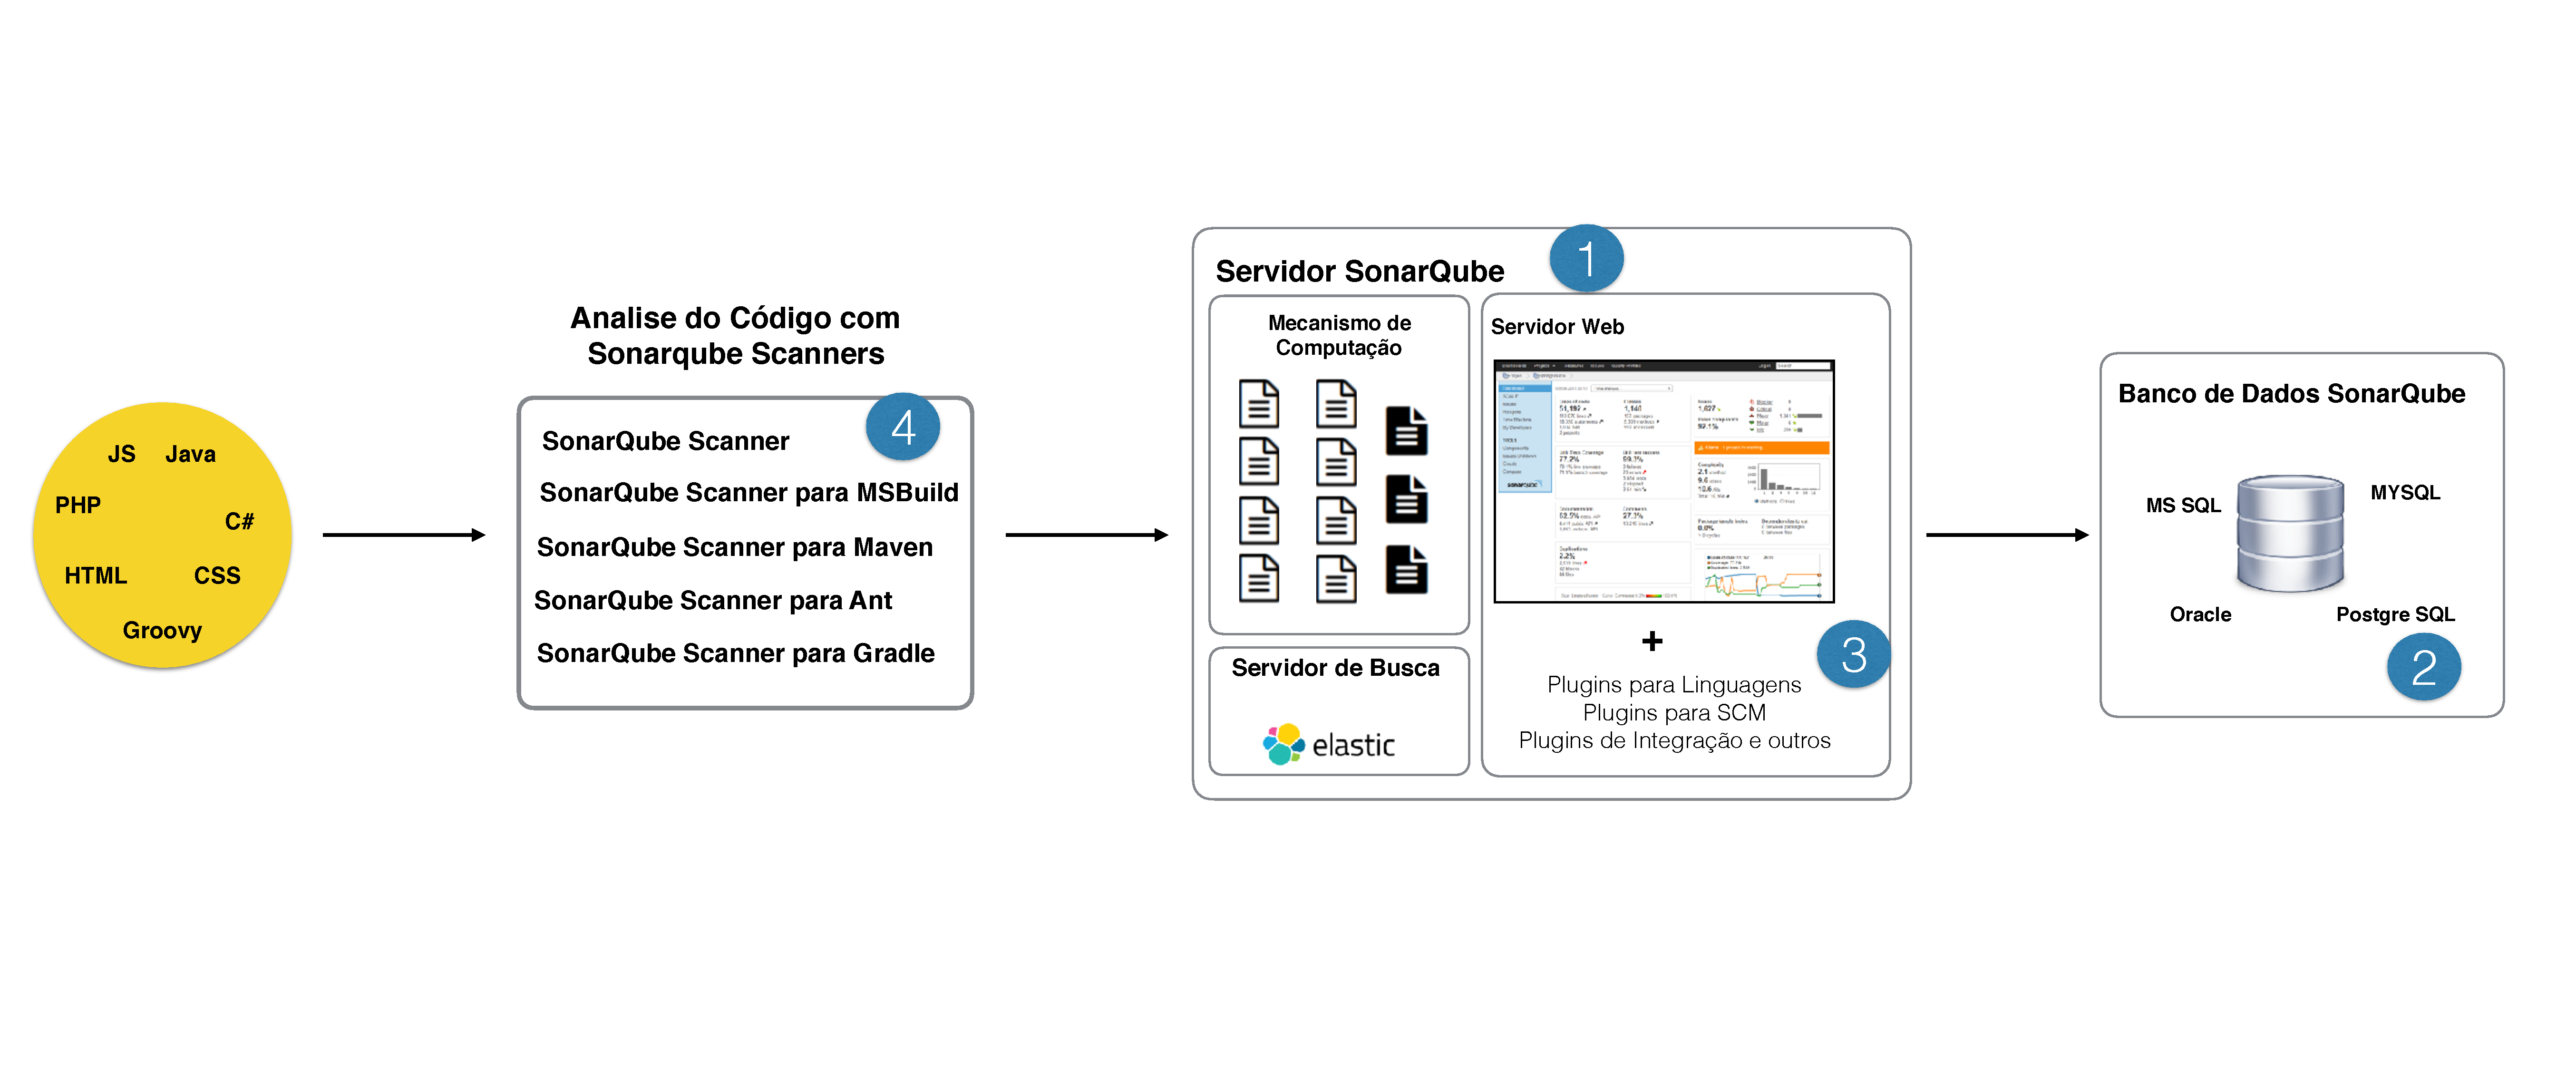
\includegraphics[scale=0.5]{Arq_Sonar}
\caption{Arquitetura SonarQube composta de quatro componentes: \cite{sonar}}
\label{img:arq_sonar}
\end{figure}
O SonarQube também é facilmente integrado com outras ferramentas utilizadas durante o ciclo de vida do software. O esquema da figura \ref{img:sonar_int} apresenta a implantação do SonarQube em diversos estágios do desenvolvimento de software \cite{sonar}.
\graphicspath{{figuras/}}
\begin{figure}[h]
\centering
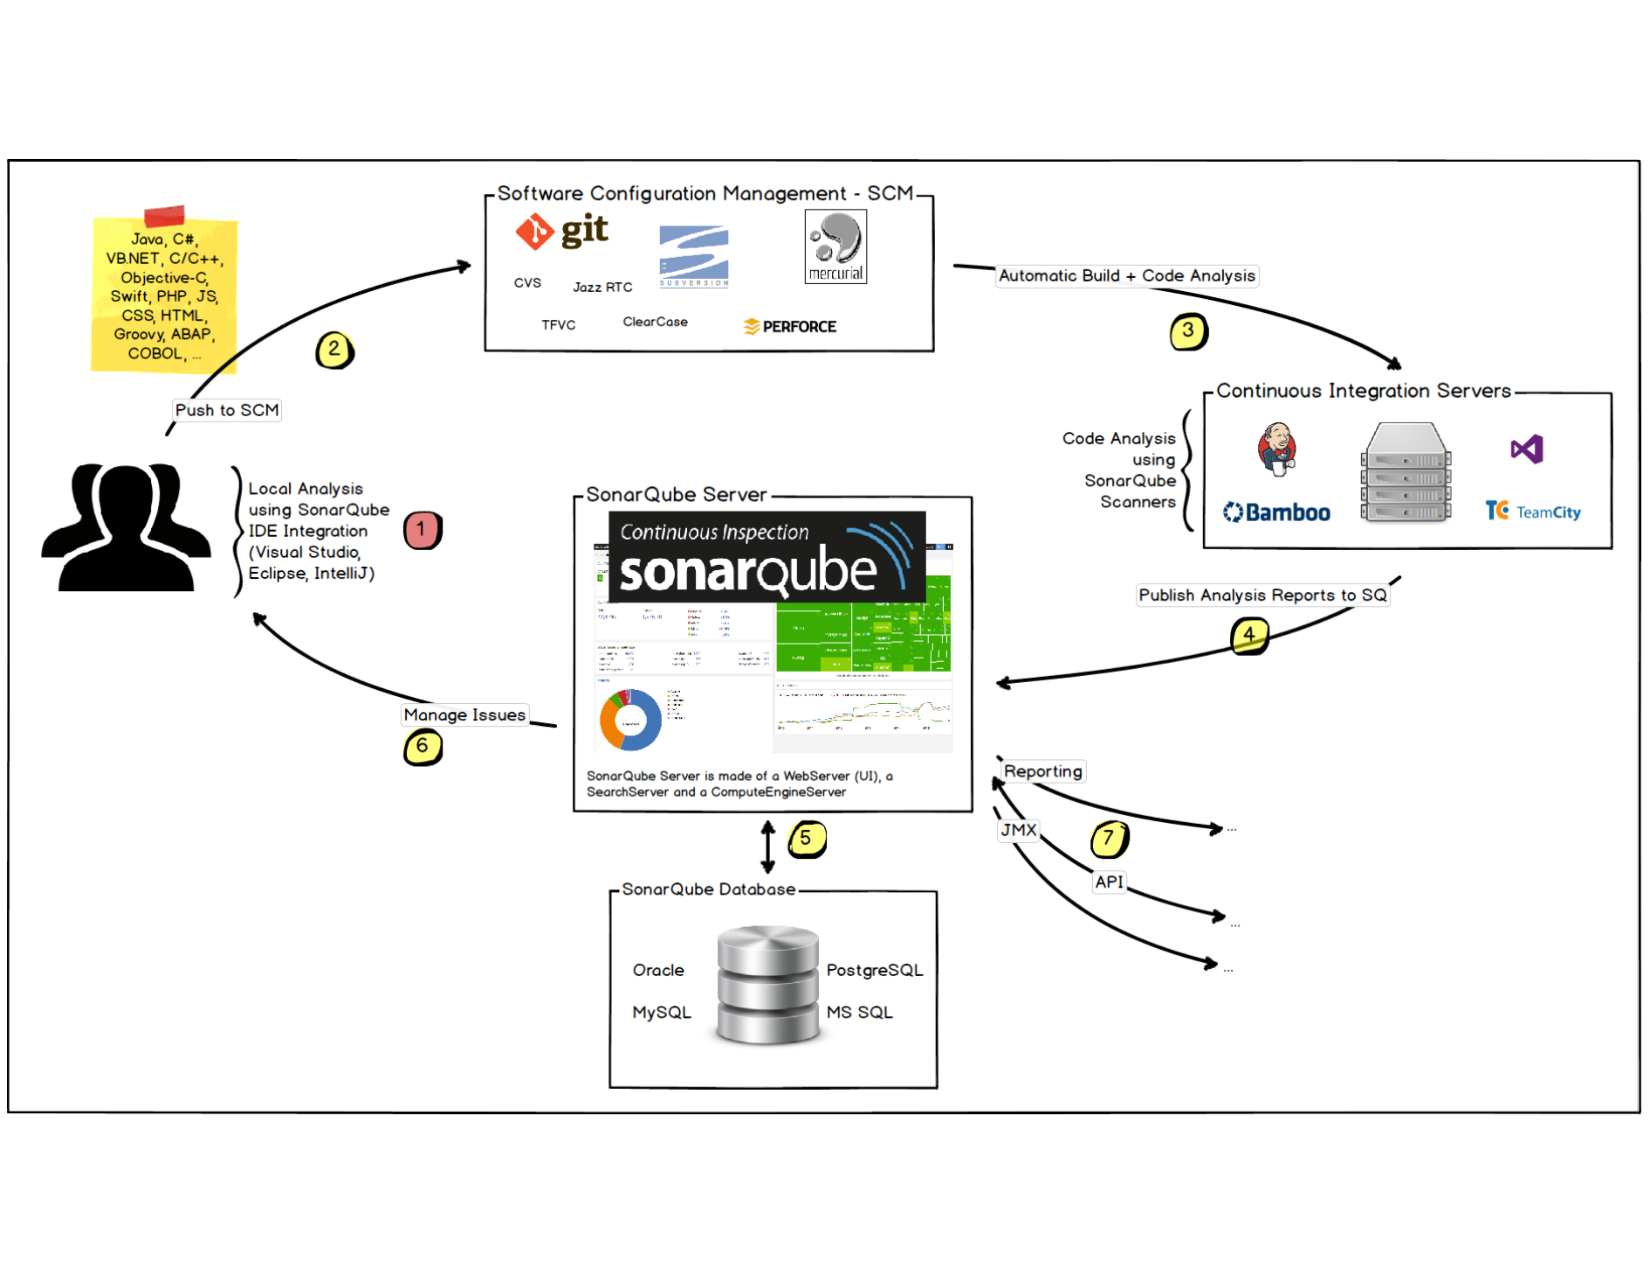
\includegraphics[scale=0.5]{sonar_int}
\caption{Integração SonarQube em Diversas Áreas de Desenvolvimento de Software: \cite{sonar}}
\label{img:sonar_int}
\end{figure}
\begin{enumerate}
\item Os desenvolvedores podem utilizar uma instância do SonarQube (SonarLint) em suas próprias IDEs para rodar uma análise local.
\item Desenvolvedores podem subir seus códigos para suas ferramentas de SCM favoritas (Git, SVN).
\item O servidor de integração contínua desencadeia uma compilação automática, e a execução do SonarQube Scanner necessário para executar a análise de SonarQube.
\item O relatório de análise é enviado para o servidor do SonarQube para processamento.
\item SonarQube Server processa e armazena os resultados do relatório de análise do banco de dados SonarQube e exibe os resultados na interface do usuário.
\item Os desenvolvedores analisam, comentam, arruman seus problemas para gerenciar e reduzir sua dívida técnica através do SonarQube UI.
\item Gestores recebem um relatório da análise
\end{enumerate}

A escolha do SonarQube como ferramenta de analise estática se deu pelo fato de que grande parte dos orgãos públicos utilizam esta ferramenta para fazer a avaliação da qualidade dos softwares entregues pelas tercerizadas. Muito dos editais encontrados neste trabalho utilizavam o SonarQube como uma das ferramentas de audição dos softwares entregues.

	
	\subsection{Google Charts e Charts.js}
	\label{sub:google_charts_chartsjs}
	O \textit{Google Charts} é uma API disponibilizada pelo Google, ela fornece uma maneira perfeita visualizar dados em um site. De gráficos de linha simples a complexa árvore hierárquica de mapas, o \textit{google charts} fornece um grande número de tipos de gráficos prontos para uso \cite{google_charts}. A forma mais comun de utilizar o \textit{google charts} é utilizando um JavaScript dentro do código HTML. Os gráficos são visualizados utilizando classes do JavaScript e são renderizados através de HTML5/SVG o que garante o funcionamento em diversos \textit{browsers}. 
	\\Outra API utilizada é a Charts.js que é uma API open-source que também utiliza a ferramenta JavaScript e renderiza os gráficos com HTML5. O principal motivo para se utilizar o Charts.JS juntamente com o Google Charts é que a API da google não fornece o gráfico de Radar o qual é utilizado neste trabalho \cite{chartsjs}.
	
\section{Ferramentas de Gerenciamento}

	\subsection{Bonita} % (fold)
	\label{sub:Bonita}
		 A ferramenta Bonita\footnote{http://www.bonitasoft.com/} foi escolhida graças a sua facilidade de utilização e portabilidade para o sistema operacional Mac OS X e o fato de ser gratuita. Esta ferramenta auxilia na modelagem de processos.
	% subsection bizagi_process_modeler (end)

	\subsection{Mac OS X} % (fold)
	\label{sub:Mac OS X}
		O sistema operacional Mac OS foi baseado no kernel Unix e fabricado e desenvolvido pela empresa Apple Inc. Utilizou-se a versão 10.11 do sistema também conhecida como "\textit{El Capitan}".
	% subsection linux_mint (end)

	\subsection{LaTeX} % (fold)
	\label{sub:latex}
	
	O LaTeX\footnote{https://www.latex-project.org/} foi desenvolvido na década de 80 cujo objetivo era simplificar a diagramação de textos científicos e matemáticos, onde atualmente dispõe de uma grande quantidade de macros para bibliografia, referencias, gráficos entre outros.
	% subsection latex (end)

	\subsection{Sublime Text 3} % (fold)
	\label{sub:sublime_text_3}
		O Sublime Text 3\footnote{https://www.sublimetext.com/3} é um editor de texto bastante utilizado por programadores, por possuir apoio para diversas linguagens de programação, incluindo textos em LaTeX.
	% subsection sublime_text_3 (end)

	\subsection{Zotero} % (fold)
	\label{sub:zotero}
		Zotero \footnote{https://www.zotero.org} é um software para gerenciamento de referências bibliográficas. Ele possui integração com o \textit{browser}, sincronização online e criação de bibliografias estilizadas.
		
		
		
	\section{Resumo do Capítulo}